%  Simo.Nikula@gmail.com
\def\mytitle{Breakable Elastic-plastic Constraint for Impulse-based Physics Engines}
\def\lut{Lappeenranta University of Technology}

\documentclass{jcgt}
\usepackage{tikz}
\usepackage{verbatim}
\usepackage[utf8]{inputenc}
\usetikzlibrary{arrows}
\usetikzlibrary{arrows.meta}
\setciteauthor{Simo Nikula, Aki Mikkola and Timo Björk}
\setcitetitle{\mytitle}

% Mark submissions with the date of submission using the following line:
%\submitted{\today}

% Once an article is accepted accepted, switch to the following line and comment the preceding one. The editor will supply the argument values.
\accepted{2014-02-07}{2014-02-07}{2014-02-07}{Editor Name}{3}{1}{1}{1}{2014}
\seturl{http://jcgt.org/published/0003/01/01/}


%%%%%%%%%%%%%%%%%%%%%%%%%%%%%%%%%%%%%%%%%%%%%%%%%


\begin{document}
\title{Breakable Elastic-plastic Constraint for\\Rigid Body Simulation}

\author
       {Simo Nikula,  Aki Mikkola, Timo Björk\\\lut
       }

\teaser{
  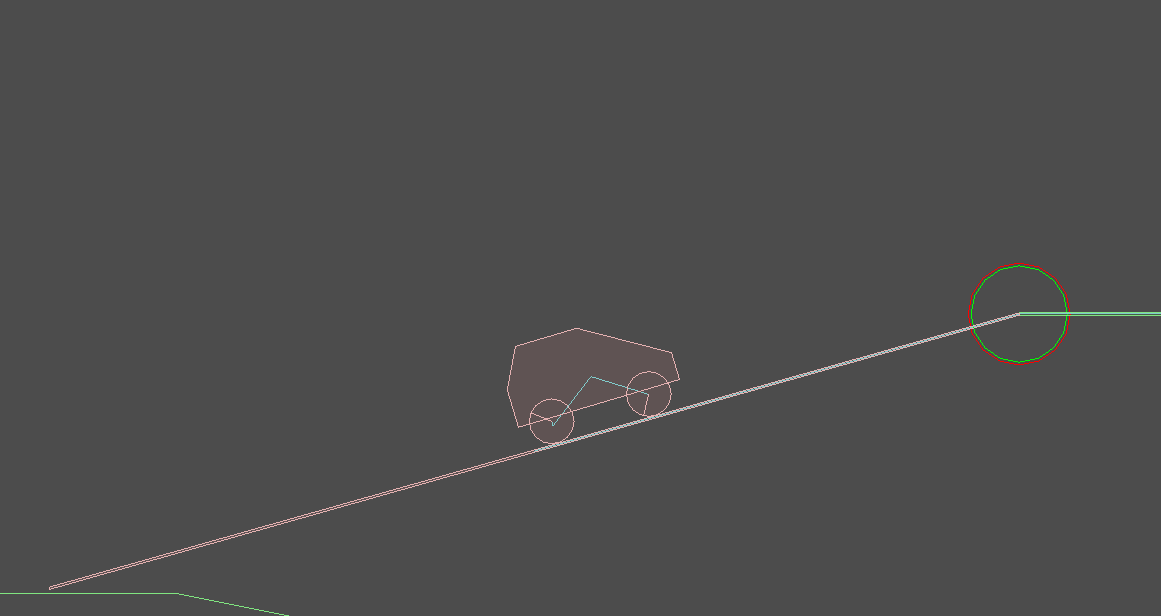
\includegraphics[width=5cm]{figs/CarAtRamp}
  \label{fig:teaser}
  \caption{Adding ductile breakable constraint to popular open source physics engine Box2D allows more realistic simulation of many scenarios. In picture above ramp is under elastic loading.}
}

\maketitle
\thispagestyle{firstpagestyle}

\begin{abstract}
\small
This paper introduces simple and efficient method to simulate ductile fracture in existing 
impulse-based physics engines.
Method is based on technique of splitting bodies to multiple pieces and joining them with constraints.
Procedure to provide realistic parameters for constraints is described.
Procedure may be based on body dimensions and material parameters or desired bahviour.

Sample program with source code are made available to allow developers already using 
Box2D to add plasticity into their simulations.
\end{abstract}



%-------------------------------------------------------------------------
\section{Introduction}
\label{sec:introduction}

Theory for handling of plasticity in computer graphics has been presented already 1988, \cite{cg1988}. 
Recent paper by Jones  provides extensive listing of related work during past decades, \cite{Jones:2016:EPD}.

In impulse-based phycis engines most breakable scenarios  are implemented by destructing various bodies based on collision
or impulse exceeding predefined limit. This provides simple means for visualization of explosions and high speed collisions 
on brittle structures.  
Nevertheless, breaking of steel or reinforced concrete structures using this approach 
is not appropriate if the simulation is to look realistic or structures should not fail completely.

More realistic simulation of ductile destructable bodies is possible but in many cases it would require 
selecting of new physics engine.

\paragraph{Our approach}
This study will introduce an approach to account for plastic deformation in impulse-based phycis engines.   
Presented methodology does not require significant software development efforts from
game vendors and is thus easily adoptable. 
In the introduced method, plastic deformation takes place if the force or moment exceeds a predefined 
limit, deformation absorbs energy and joint breaks if plastic capacity is exceeded. 
Maximum forces and moments can be estimated based on the plastic section modulus or
by defining maximum elastic displacement or based on desired capacity.
Joint breaking is based on summing plastic deformation and comparing it to a
predefined material and geometry based limit. The elastic part of deformation is modelled by employing 
modification of an existing constraints. 

This paper follows idea of
allowing game designers to get desired behaviour without diving into details of structural engineering.
Idea was presented by Catto, \cite{ecsc}. Basic idea is that game designer selects spring frequency so that
integration is stable. Downside is that constraints will be quite soft. In our method game designers get new option
to use rigid-plastic constraints.

\paragraph{Limitations}
Forces are calculated by dividing impulse by timestep and maximum impulse is calculated
by multiplying maximum force by timestep. 
This means that simulation of quick interactions requires small timestep.
This limitation is not introduced by this approach but is build in feature of impulse-based simulation.
We discuss few methods to maximize realisticy of simulation of collisions but this issue will need further work.
Bending moment - normal force interactions and multiaxial stress are not taken into account. 
Simulation of many bodies connected by constraints has convergence issues which will also need further work.

\section{Description of plasticity in the framework of physics engines}

In this work simulation of breaking of bodies made of ductile material is made more realistic 
by splitting the rigid body
to multiple bodies that are connected by energy absorbing joints.

\paragraph{Stress-strain behaviour of ductile steel}
A typical engineering stress-strain curve of ductile steel is shown in Figure \ref{fig:sscurve}.

\begin{figure}
\centering
\begin{tikzpicture}
\coordinate (Y) at (1,4);
\draw[->] (0,0) -- (6,0) node[right] {\large{$\epsilon$}};
\draw[->] (0,0) -- (0,5) node[above] {\large{$\sigma$}};
\draw(0,0) -- (Y) -- (2,4) .. controls (5,5) .. (6,4);
\draw[dashed](0,4) -- (Y);
\node at (-0.2,4) [align=right] {$f_y$};
\draw(0.25,1) -- (0.5,1) -- (0.5,2);
\node at (0.75,1.5) {$E$};
\node at (0.8,2.5) [anchor=west] {$\sigma = E \epsilon$ if $\sigma \le f_y$};
\end{tikzpicture}
\caption{Engineering stress-strain curve of ductile steel (not to scale).}
\label{fig:sscurve}
\end{figure}

In Figure \ref{fig:sscurve}, $\sigma$ is stress, $E$ is Youngs modulus and $f_y$ is yield stress.
Engineering stress and strain mean that original dimensions are used in stress calculation,
\cite{dowling}.
%\citet[p.~108]{dowling}.
The stress-strain curve is not drawn to scale as elastic strain could not be seen as it is typically 
0.001 to 0.005 and fracture strain can be 100 times larger.
In practice this means that elastic displacement due to axial forces is usually not visible.
Visible elastic displacement is usually due to bending.

In this work, an elastic-fully plastic material model is used in most scenarios.
Having elastic part allows elastic displacements for slender structures. 
Elastic material behavior is ignored in approach introduced in this work if
the deformation is related to a higher frequency
than integration stability would allow.
It should be noted that geometry
of bodies is not updated during analysis and thus engineering stress-strain properties are used.

In this work, strain hardening is taken into account by assuming that plastic volume in bending
expands, 
\cite{dowling}.
%\citet[p.~672]{dowling}.
Material that starts to yield first is hardened and as a result of which yielding moves.
%
The difference between the elastic and plastic section modulus is depicted in Figure \ref{fig:wp}.

\begin{figure}[htb!]
\centering
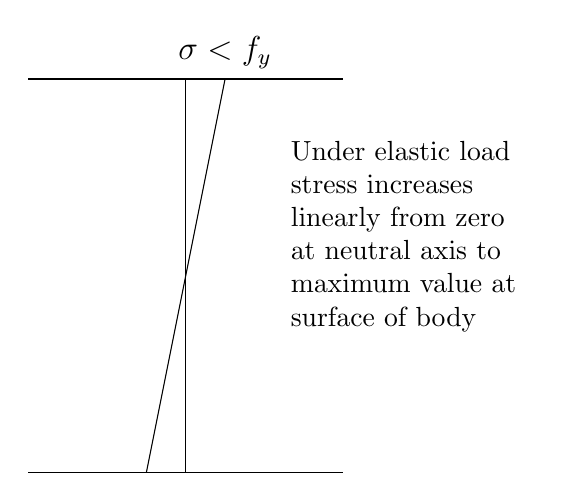
\begin{tikzpicture}
\coordinate (S) at (2.5,5);
\draw (0,5) -- (4,5) ;
\draw (0,0) -- (4,0) ;
\draw (2,0) -- (2,5) ;
\draw (1.5,0) -- (S); 
\node[above] at (S) [align=center] {\large{$\sigma<f_y$}};
\node[anchor=west] at (3,3) {
\begin{tabular}{l}
Under elastic load\\
stress increases\\
linearly from zero\\
at neutral axis to\\
maximum value at \\
surface of body
\end{tabular}
};
\end{tikzpicture}
\hspace{1cm}
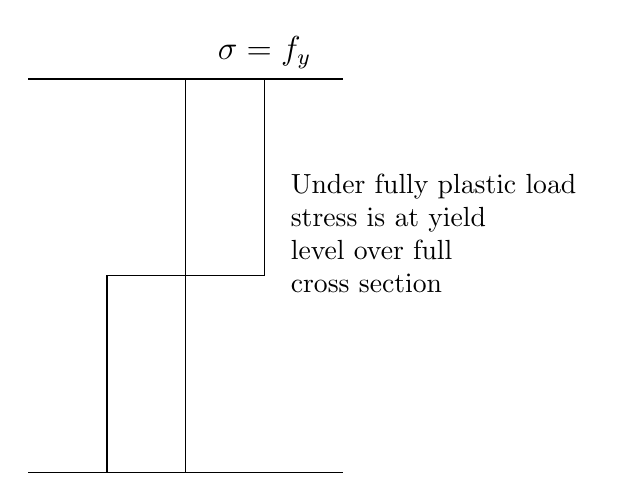
\begin{tikzpicture}
\coordinate (S) at (3,5);
\draw (0,5) -- (4,5) ;
\draw (0,0) -- (4,0) ;
\draw (2,0) -- (2,5) ;
\draw (1,0) -- (1,2.5) -- (3,2.5) -- (S); 
\node[above] at (S) [align=center] {\large{$\sigma=f_y$}};
\node[anchor=west] at (3,3) {
\begin{tabular}{l}
Under fully plastic load\\
stress is at yield\\
level over full\\
cross section
\end{tabular}
};
\end{tikzpicture}
\caption{Axial stress distribution over a cross section for bending under elastic and fully plastic loads.}
\label{fig:wp}
\end{figure}

As shown in Figure \ref{fig:wp}, if stress is below yield limit $f_y$, stress and strain are linear within the material.
If cross section is fully plastic, stress is assumed to be at yield level over the whole cross section such that 
the plastic section modulus is higher than the elastic section modulus.

\paragraph{Plastic capacities based on dimensions and material}
In this work, plasticity is handled by defining maximum forces using plastic capacities, which are defined below.

Maximum force acting in a direction of $\vec{r}_{anc}^{\,i} $
is product of area and yield stress as follows:

\begin{equation} \label{eq:fN}
N_{max}= \int_A f_y.
\end{equation}

Maximum forces acting perpendicular to $\vec{r}_{anc}^{\,i} $
are a product of area and shear yield stress $\tau_y$ as follows:
\begin{equation} \label{eq:fQ}
Q_{max}= \int_A \tau_y.
\end{equation}

Maximum moment is integral of the perpdendicular distance 
and yield stress $f_y$ as given for the moment around  the $z$-axis:

\begin{equation} \label{eq:Mz}
M_{max}^z= \int_A x f_y.
\end{equation}


Maximum forces and moments for a
rectangular section with width $b$ and height $h$ using constant yield stress
are given in Table \ref{tab:maxForces}.
Yield shear stress is assumed to be $ 0.5\, f_y$ using the Tresca yield critetion.
If the von Mises yield criterion is used 0.5 is replaced by 0.58 ($1/\sqrt{3}$), \cite{dowling}.
% p. 262, p. 268
These are not exact values in a multiaxial stress state but they
should be acceptable in most gaming scenarios.

\begin {table}
\small
\begin{center}
\begin{tabular}{| c| c|}
\hline
{\bf Direction} & {\bf Maximum value}  \\ \hline
maximum shear force & $0.5\, b\, h f_y$ \\ \hline
maximum normal force & $b\, h\, f_y$  \\ \hline
maximum bending moment in direction of $h$& $0.25\, b\, h^2 \, f_y$  \\ \hline
\end{tabular}
\end{center}
\caption{Maximum forces and moments for 
rectangular section with width $b$ and height $h$ using constant yield stress $f_y$}
\label{tab:maxForces} 
\end {table}

\paragraph{Plastic capacities based on desired behaviour}
Capacities can also be defined directly based on desired scenarios.
E.g. joints for bridge can designed so that maximum shear force is larger than
weight of heaviest vehicle so that all vehicles can drive to bridge. Maximum 
bending moment could be set so that joint will start to rotate when heaviest vehicle is
near the middle of bridge.

For elastic-plastic cases maximum capacity can also be defined by setting maximum elastic 
displacement or rotation.

\paragraph{Joint breaking}
Joint breaking is based on summing of plastic displacement or rotation.
Process can be subdivided few phases.

\begin{enumerate}
\item Hitting maximum impulse value triggers additional processing.
\item New neutral position is calculated so that elastic part is subtracted from current position.
\item Plastic strain or rotation is incremented.
\item Current plastic strain or rotation is compared to maximum value and joint is broken if 
current value exceeds predefined maximum value. This part can be finetuned e.g. so that joint is 
not broken during compression if connected parts are made of material which can handle large
strains due to compressive forces. 
\end{enumerate}

\paragraph{Joint breaking in one simulation step} High velocity collisions may cause joints to break within one step.
In such cases joints can cause too large impulse as shown in  Figure~\ref{fig:tippingCar}.

\begin{figure}[htb]
  \centering
   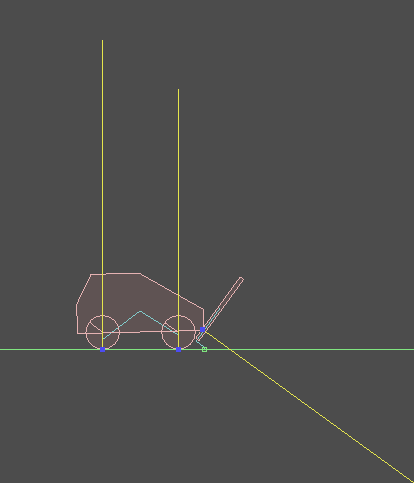
\includegraphics[height=5cm]{figs/tippingCar1.png}
   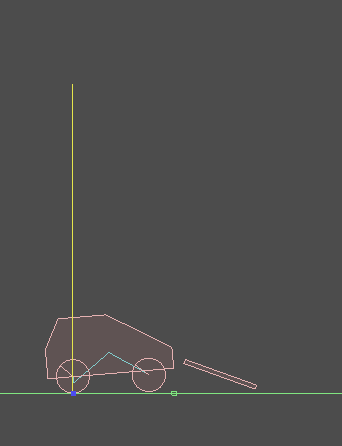
\includegraphics[height=5cm]{figs/tippingCar2.png}
   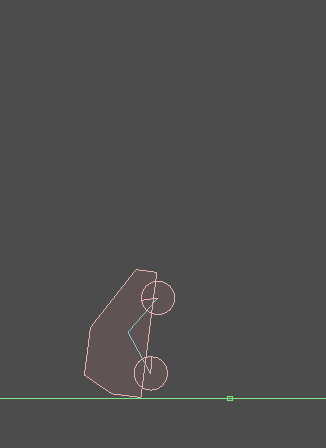
\includegraphics[height=5cm]{figs/tippingCar3.png}
   \caption{\label{fig:tippingCar}
     Large impulse turns car over.}
\end{figure}
Making simulation step smaller is not desired solution.
In this paper following procedure suggested.

\begin{enumerate}
\item At start of each step predict outcome of current step for each joint using current velocities and
maximum and current strains and rotations.
\item If current impulse is about to break constraint within current step scale down maximum impulse
so that joint does not exceed planned capacity. 
\end{enumerate}

\paragraph{Impulse initialization}
Joint impulses should be initialized using suitable methods to minimize errors.

\section{Implementation for Box2D}
b2ElasticPlasticJoint implementation is based on b2WeldJoint which implements rigid and flexible joints as
described in Catto's paper~\shortcite{ecsc} on soft constraints. Main idea is that game designer should not have
to find suitable values to get desired functionality but constraint is configured by giving desired  damping ratio and frequency.
This principle leads in many cases to quite soft constraints to keep simulation stable. 
b2WeldJoint supports also rigid joint in which case iterative solver creates some flexibility.
If maximum forces and moment are set to very high value b2ElasticPlasticJoint behaves like b2WeldJoint but is slighly slower.

\paragraph{Changes to processing} 
In addition to allowing definition of maximum forces and moment during initialization 
b2ElasticPlasticJoint allows definition of maximum moment by giving maximum elastic rotation.

For each step maximum rotational impulse and linear impulses are calculated using step length and 
current orientation of the joint.

During solution phase impulse is clamped so that it does exceed predefined limit.
If clamping is activated additional processing is done at the beginnig of next step to update neutral position and
increment plasticity values.

\paragraph{Debugging tools} 
Box2D testbed offers many useful tools and only few additions were made for testing of plasticity.
\begin{enumerate}
\item Tunable visualization of joint forces
\item Numerical output of joint forces as absolute values and as percentage of maximum forces
\item Numerical output of usage of plastic capacity
\item Selection of joints for display of numerical values
\end{enumerate}

\section{Examples} 

\subsection{Cantilever beam} 

\subsection{Multifloor frame} 

\subsection{Car} 
Dynamic bodies are car (680 kg), wheels (50 kg for each axel), and ramp (2160 kg). 
Ramp is joined to fixed part with b2ElasticPlasticJoint having frequency of 1 Hz.
Maximum elastic rotation is set to 0.12 and maximum plastic rotation to 0.4.
With this configuration own weight of ramp uses about 13 \% of plastic capacity during initialization phase.
After first jump about 50 \% of  plastic capacity is used. Each additional jump uses about 
7 \% of plastic capacity.


\small
\bibliographystyle{jcgt}
\bibliography{ref}

\section*{Index of Supplemental Materials}

\begin{enumerate}
\item Box2D source with plasticity extensions 
 \href{https://github.com/simo-11/Box2D}{https://github.com/simo-11/Box2D}

\end{enumerate}

\section*{Author Contact Information}

\hspace{-2mm}\begin{tabular}{p{0.3\textwidth}p{0.3\textwidth}p{0.3\textwidth}}
Simo Nikula\newline
\href{mailto:Simo.Nikula@gmail.com}{Simo.Nikula@gmail.com}
&
Aki Mikkola\newline
\href{mailto:Aki.Mikkola@lut.fi}{Aki.Mikkola@lut.fi}
&
Timo Björk\newline
\href{mailto:Timo.Bjork@lut.fi}{Timo.Bjork@lut.fi}
\end{tabular}


\afterdoc

\end{document}
